\documentclass[12pt]{article}

%%%%%%%%%%%%%%%%%%%
% Packages/Macros %
%%%%%%%%%%%%%%%%%%%
\usepackage{amssymb,latexsym,amsmath}     % Standard packages
\usepackage{graphicx}
\usepackage{subcaption}
%\usepackage{subfig}
%\usepackage[caption=false]{subfig}
\usepackage{cite} % Allows for ranges in citation
\usepackage{mciteplus}
\usepackage[toc,page]{appendix}
\usepackage{titlesec}
\usepackage{xcolor}
\usepackage{hyperref}    % Hyperlinks in references
%\usepackage[all]{hypcap} % Internal hyperlinks to floats.
\definecolor{darkblue}{rgb}{0,0,0}
\definecolor{darkgreen}{rgb}{0,0.5,0}
\definecolor{darkviolet}{rgb}{0.55,0.,0.55}
\hypersetup{colorlinks=true, linkcolor=darkblue, citecolor=darkviolet, urlcolor=blue}
\usepackage{array}
\usepackage{booktabs}
%%%%%%%%%%%
% Margins %
%%%%%%%%%%%
%\addtolength{\textwidth}{2.3in}
%\addtolength{\textheight}{2.3in}
%\addtolength{\evensidemargin}{-0.2in}
%\addtolength{\oddsidemargin}{-0.2in}
%\addtolength{\topmargin}{-1.2in}
%\usepackage[usenames,dvipsnames,svgnames,table]{xcolor}

%%%%%%%%%%%%%%%%%%%%%%%%%%%%%%
% Theorem/Proof Environments %
%%%%%%%%%%%%%%%%%%%%%%%%%%%%%%
\newtheorem{theorem}{Theorem}
\newenvironment{proof}{\noindent{\bf Proof:}}{$\hfill \Box$ \vspace{10pt}}  


%%%%%%%%%%%%
% Document %
%%%%%%%%%%%%
\begin{document}

\title{\textit{GateParamterisedPinholeCollimator} class for simulation of preclinical SPECT}
\author{Olga Kochebina (kochebina@gmail.com)}
\maketitle
\tableofcontents
\newpage
%\begin{abstract}
%\end{abstract}



\pagebreak


%%%%%%%%%%%%%%%%%%%%%%%%%%%%%%%%%%%%%%%%%%%%%%%%%%%
\section{Introduction}
The GateParametrisedPinholeCollimator class was developed for GATE simulations of a multiple pinhole collimator for preclinical SPECT imaging.
In the simulation we use analytical model for the collimator geometry description.

An example of preclinical SPECT with a multipinhole collimator is a nanoSPECT/CT by Mediso shown in Figure~\ref{fig:scanner} and macros can be found in \href{https://github.com/kochebina/ParametrisedPinholeCollimator/tree/main/macros}{macros on github}. It is a four head system with exchangeable collimators adapted to imagning subject. An example of pinhole collimator simulated with GATE is presented in Figure~\ref{fig:colli}.
 
\begin{figure}[htp]
\centering
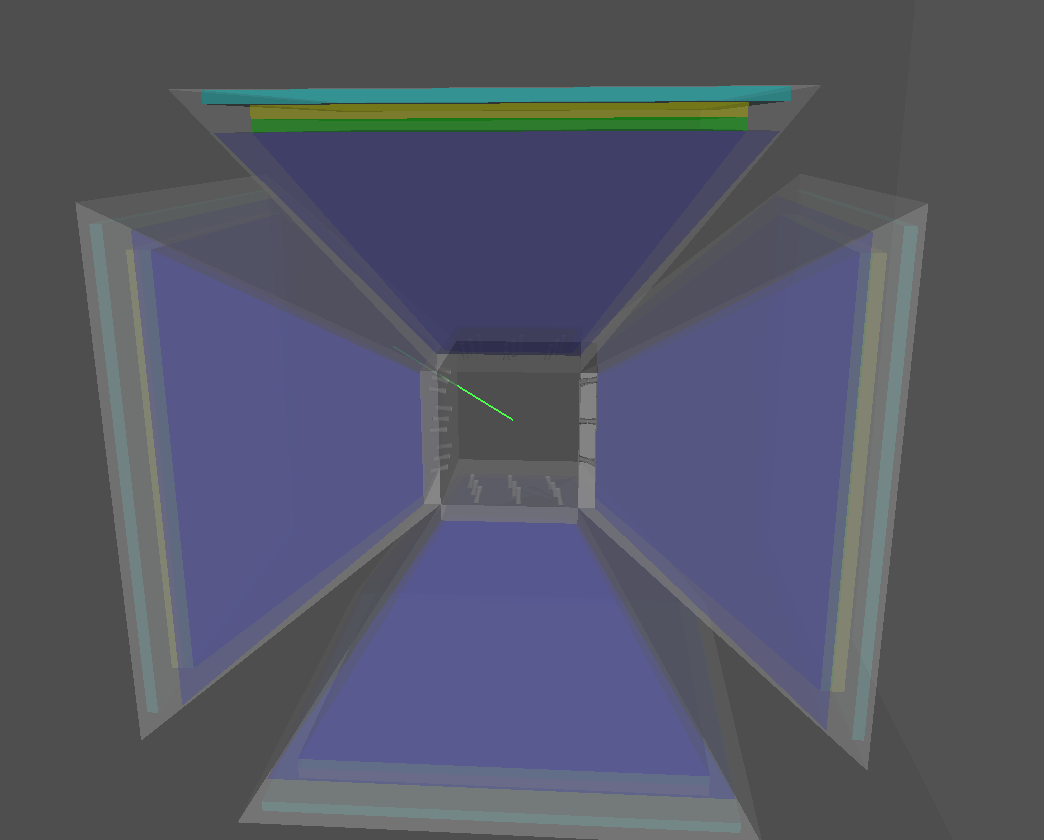
\includegraphics[scale=0.3]{figs/scanner.png}
\caption{Illustration for simulated nanoSPECT}
\label{fig:scanner}
\end{figure}

\begin{figure}[htp]
\centering
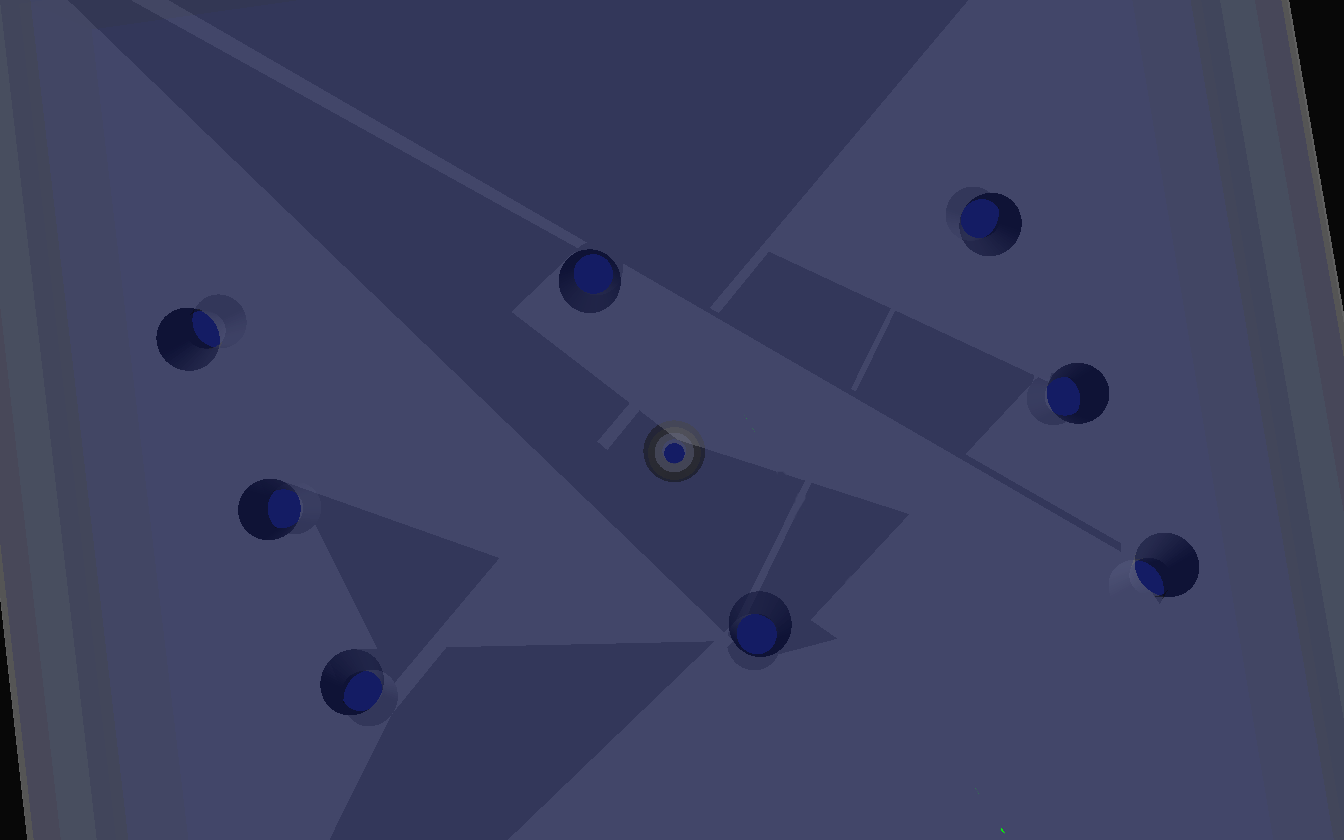
\includegraphics[scale=0.3]{figs/colli.png}
\caption{Illustration for pinhole collimator}
\label{fig:colli}
\end{figure}


\section{Options and input data}
The geometry of pinhole is defined from a G4-pyramid with a subtracted cones (G4Cons) in order to have pinholes drilled from both sides of a collimator plane.

The pyramid is defied with mac options:  
\begin{verbatim}
/gate/colli/geometry/setDimensionX1 80 mm
/gate/colli/geometry/setDimensionY1 84 mm
/gate/colli/geometry/setDimensionX2 80 mm
/gate/colli/geometry/setDimensionY2 84 mm
/gate/colli/geometry/setHeight 10 mm
\end{verbatim}

The collimator rotation radius, i.e. distance from the center of field of view to the pinholes center (see Figure~\ref{fig:rot_radius} and Figure~\ref{fig:pinhole}) is defined as:
\begin{verbatim}
/gate/colli/geometry/setRotRadius 45 mm
\end{verbatim}

\begin{figure}[htp]
\centering
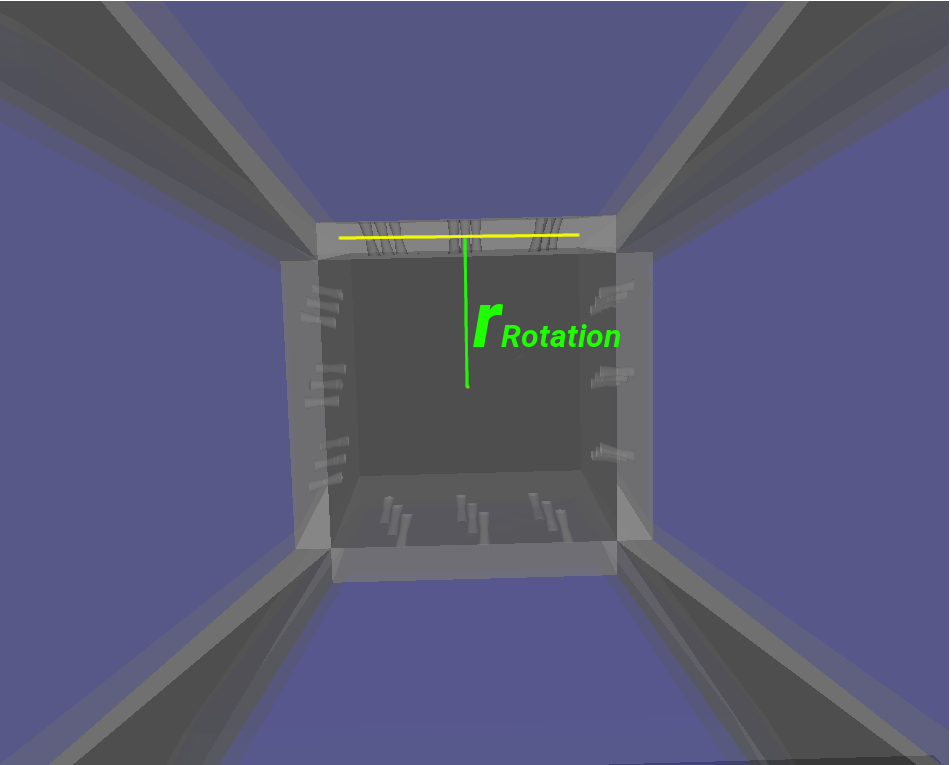
\includegraphics[scale=0.3]{figs/rot_radius.png}
\caption{Definition of the rotation radius}
\label{fig:rot_radius}
\end{figure}


The pinholes are defined with an option file:
\begin{verbatim}
/gate/colli/geometry/input mac/APT2.pin
\end{verbatim}

The stricture of the option file, APT2.pin, is the following (an example could be found in Table~\ref{tab:ResTUBES}):
\begin{verbatim}
Number of pinholes
x	y	diameter cone_angle	x_focal y_focal
\end{verbatim}

 \begin{table}[ht]
 \begin{center}
     \begin{tabular}{cccccc}
      \#~~ x & y & dia & alpha cone & $x_{focal}$ & $y_{focal}$ \\
	  {[APT2]} &  & &  &  &  \\
	   9 &  & &  &  &  \\
	   28.898 & 11.949 & 2.5 & 7.5 & 20.0002 & 0 \\
		25.19 & 0 & 2.5 & 7.5 & 15.0274 & 0 \\
		21.464 & -11.949 & 2.5 & 7.5 & 10.0315 & 0 \\
		3.743 & 11.949 & 2.5 & 7.5 & 5.01876 & 0 \\
		0     & 0 & 2.5 & 7.5 & 0 & 0 \\
		-3.743 & -11.949 & 2.5 & 7.5 & -5.01876 & 0 \\
		-21.464 & 11.949 & 2.5 & 7.5 & -10.0315 & 0 \\
		-25.19 & 0 & 2.5 & 7.5 & -15.0274 & 0 \\
		-28.898 & -11.949 & 2.5 & 7.5 & -20.0002 & 0 \\
     
     \end{tabular}
     \caption{Example of APT2.pin option file}
     \label{tab:ResTUBES}
  \end{center}
  \end{table}
In Table~\ref{tab:ResTUBES} one can find a description of a collimator called "APT2" with 9 holes. The diameter of pinholes (at the center) is 2.5~mm, the opening cone angle ($\alpha$) is 7.5~degree. The x and y coordinates are the centers of the pinholes. The focal coordinates are illustrated in Figure~\ref{fig:pinhole}.
\begin{figure}[htp]
\centering
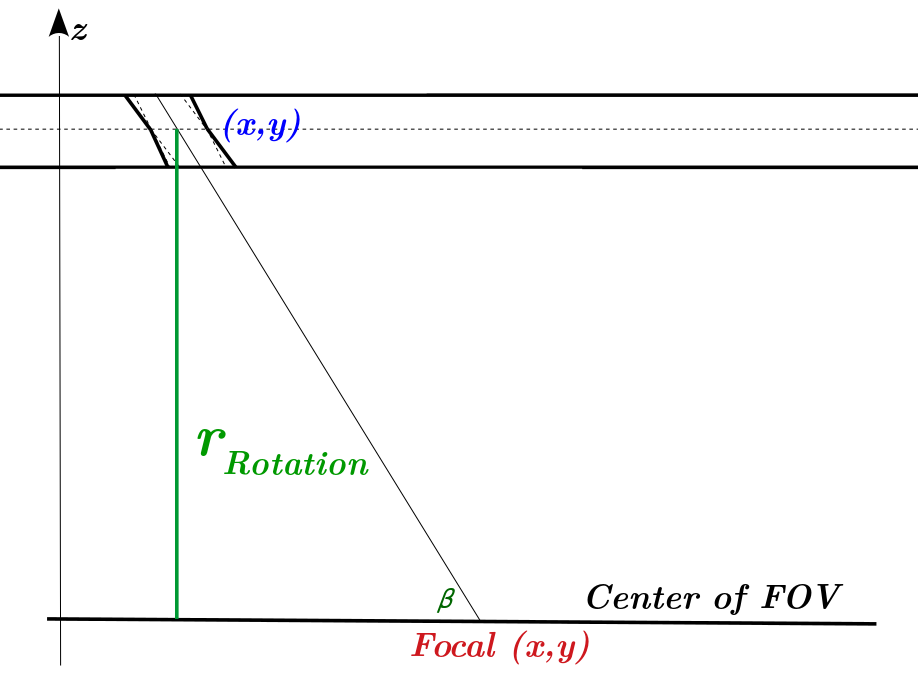
\includegraphics[scale=0.4]{figs/pinhole_for_option_file.png}
\caption{Illustration of parameters defined in APT2.pin option file}
\label{fig:pinhole}
\end{figure}


\clearpage
\section{Pinhole geometry calculations}
The result of the following calculations is implemented in GateParametrisedPinholeCollimator class.

The names of the variables in the class are the same as in Figures~\ref{fig:fig_def_size} and ~\ref{fig:fig_def_positions} and the calculations below. The final results used in the GateParametrisedPinholeCollimator are framed.

\

The drilled cones of pinholes are simulated as G4Cons. The required and nontrivial parameters are: 
\begin{itemize}
\item Geometrical cone parameters
	\begin{itemize}
	\item height of the cone, \textit{Dz} 
	\item radius of the cone basis, \textit{rmax}
	\end{itemize}	
\item Cone tilt 
\item Displacement correction due to tilt
	\begin{itemize}
	\item  on \textit{x} (\textit{x} = the first column read from .pin file) : $x+\Delta x$ for "down cone" or $x-\Delta x$ for "upper cone"
	\item on \textit{y} (\textit{y} = the second column read from .pin file): $y+\Delta y$ for "down cone" or $y-\Delta y$ for "upper cone"
	\item on \textit{z} (\textit{z} = collimator rotation radius, Figure~\ref{fig:rot_radius}) : $-\Delta z$ for "down cone" or $\Delta z$ for "upper cone" 
	\end{itemize}	
\end{itemize}


\subsection{Geometrical cone parameters}

The known parameters are: \textbf{\textit{d ( = dia)}} -- diameter of the pinhole, $\mathbf{\alpha}$ = cone opening angle, \textit{x} and \textit{y} -- center of pinhole, $x_{focal}$ and $y_{focal}$ -- focal coordinates, \textit{z} = rotation radius, \textit{h} = half of a thickness of collimator plate.

\begin{figure}[htp]
\centering
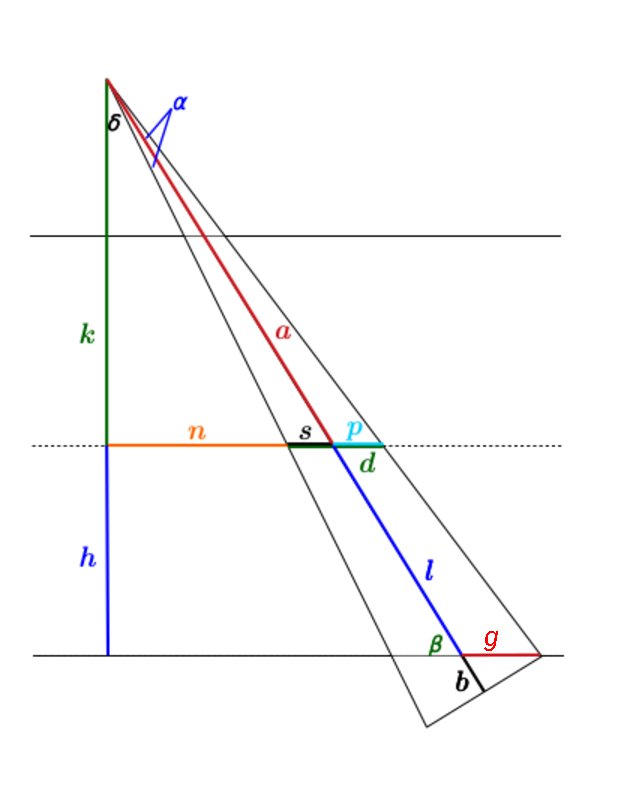
\includegraphics[scale=1]{figs/fig_def_size.pdf}
\caption{Illustration for pinhole size parameter definitions}
\label{fig:fig_def_size}
\end{figure}
\begin{enumerate}
\item Calculation of $\beta$	
	  \begin{equation} 	
	\boxed{\beta=|\pi/2- atan(|x-x_{focal}/z|)|}
	\end{equation}

\item Calculation of $l$				
	$$l=\frac{h}{\cos(\delta+\alpha)}=\frac{h}{\sin\beta}$$
	  \begin{equation} 	
	\boxed{l=\frac{h}{\sin\beta}}
	\end{equation}
\item Calculation of $k$ and $n$
	$$\delta=90^{o}-(\alpha+\beta)$$

	\[
	\left \{
	\begin{array}{c @{=} c}
    \tan\delta = \frac{1}{\tan(\alpha+\beta)}& \frac{n}{k} \\
   	\tan(\delta+2\alpha) = \frac{1}{\tan(\beta-\alpha)} & \frac{n+d}{k} \\
	\end{array}
	\right.
	\]
	
	\[
	\left \{
	\begin{array}{c @{=} c}
    \tan(\alpha+\beta)& \frac{k}{n} \\
   	\tan(\beta-\alpha) & \frac{k}{n+d} \\
	\end{array}
	\right.
	\]
	
%	$$n=\frac{d\cdot\tan(\beta-\alpha)}{\tan(\alpha+\beta) - 	\tan(\beta-\alpha)}	$$	
	
\begin{equation} 	
	\boxed{k=\frac{d\cdot\tan(\beta-\alpha)\cdot\tan(\alpha+\beta)}{\tan(\alpha+\beta) - 	\tan(\beta-\alpha)}}
\end{equation}	
\begin{equation} 	
	\boxed{n=\frac{k}{\tan(\beta-\alpha)} - d}
	\end{equation}	
		
%and
%\begin{equation} 		
%  \boxed{k_{central}=\frac{d}{2\cdot\tan\alpha}}
%  	\end{equation}	
%  \begin{equation} 		
%	\boxed{n_{central}=0	}
%	\end{equation}	
%	
\item Calculation of $a$ from $k$
	$$a=\frac{k}{\cos(\delta+\alpha)}=\frac{k}{\sin\beta}$$
	  \begin{equation} 	
	\boxed{a=\frac{k}{\sin\beta}}
	\end{equation}

\item Calculation of $s$ and $b$ 
	$$\tan(\delta+\alpha)=\frac{1}{\tan{\beta}} =\frac{n+s}{k}$$
	  \begin{equation} 	
	\boxed{s=\frac{k}{\tan{\beta}}-n}
	\end{equation}
	$$p=d-s$$
	$$\frac{p}{g}=\frac{a}{a+l}$$
	$$g=\frac{(d-s)\cdot(a+l)}{a}$$ 
	$$\cos\beta=\frac{b}{g}$$
	  \begin{equation} 	
	\boxed{b=\frac{(d-s)\cdot(a+l)\cdot\cos\beta}{a}}
	\end{equation}
\item Calculation of $Dz$ for a chosen direction ($x$ or $y$)
\begin{equation} 
	\boxed{Dz_x=a+l+b}			
\end{equation}
\begin{equation} 
	\boxed{Dz_y=\frac{y-y_{focal}}{\cos{((y-y_{focal})/z)} }}			
\end{equation}	
\item In 3D: 
\begin{equation} 
	\boxed{Dz=\sqrt{Dz_{x}^{2}+Dz_{y}^{2}}}		
\end{equation}

\item Cone radius: 
\begin{equation} 
	\boxed{rmax=Dz\cdot\tan{\alpha}}			
\end{equation}
	
\end{enumerate}



\subsection{Cone tilt}

The tilt is defined with G4RotationMatrix by methods rotateX(\textit{rotX}) and rotateY(\textit{rotY}).

\begin{enumerate}
\item Definition of t
	\begin{equation} 
	t=(x-x_{focal})^2+(y-y_{focal})^2+z^2		
	\end{equation}
\item Definitions of normal \textit{x}, \textit{y} and \textit{z}
	\begin{equation} 
	x_{normal}=(x-x_{focal})/\sqrt{t}		
	\end{equation}
	\begin{equation} 
	y_{normal}=(y-y_{focal})/\sqrt{t}			
	\end{equation}
	\begin{equation} 
	z_{normal}=z/\sqrt{t}		
	\end{equation}

\item Definitions of \textit{rotX} and \textit{rotY}
	\begin{equation} 
	\boxed{rotX=atan(x_{normal}/z_{normal})}	
	\end{equation}
	\begin{equation} 
	\boxed{rotY=-atan(y_{normal}/z_{normal})}	
	\end{equation}
 \end{enumerate}
 
 
 
\subsection{Displacement correction due to tilt}
 
\begin{figure}[htp]
\centering
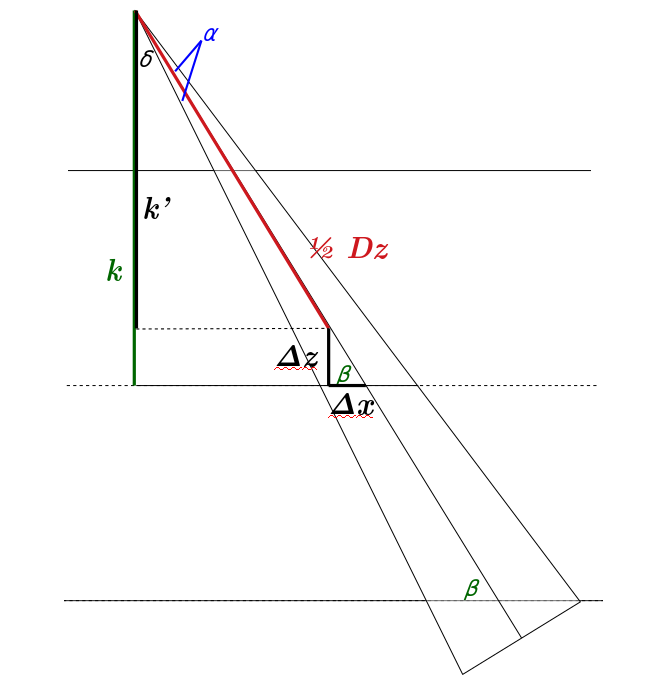
\includegraphics[scale=0.5]{figs/fig_def_positions.png}
\caption{Illustration for pinhole positions definitions}
\label{fig:fig_def_positions}
\end{figure}
According to illustration in Figure~\ref{fig:fig_def_positions} one obtains: 
\begin{enumerate}
\item Calculation of $\Delta z$
	\begin{equation} 
	\Delta z = k-k'		
	\end{equation}
	\begin{equation} 
	\cos{(\delta+\alpha)} = \sin{\beta} = \frac{k'}{Dz/2}	
	\end{equation}
	\begin{equation} 
	k' = (Dz/2)\cdot\sin{\beta} 
	\end{equation}
	\begin{equation} 
	\boxed{\Delta z = k - (Dz/2)\cdot \sin{\beta} }		
	\end{equation}
\item Calculation of $\Delta x$ or $\Delta y$ in 3D with $\phi$ as an azimuthal angle:
	\begin{equation} 
	\boxed{\Delta x = \sin{\phi}\frac{\Delta z}{\tan{\beta}}}
	\end{equation}
	\begin{equation}	
	\boxed{\Delta y =\cos{\phi} \frac{\Delta z}{\tan{\beta}}}		
	\end{equation}
\end{enumerate}
\clearpage

\section{How to obtain .pin file}
One of tricky steps is to obtain the .pin file, i.e. pinhole parameters: positions, diameters, cone opening angles and focal points positions. 

\subsection{Input from HiSPECT reconstruction software}
Here one can find a description of how it was done for one of projects where the simulation of nanoSPECT/CT by Mediso was done with GATE. It is four head camera with several pinhole exchangeable collimators. In our case we were interested in APT1, a collimator for mouse imagning, and APT2, a collimator for rat imagning. 

The best way that we found was to search information in integrated reconstruction software of the scanner. In our case it was \textbf{HiSPECT}.
The pinhole information was stored in (Figure~\ref{fig:HiSPECT4det})
\begin{verbatim}
Scivis/HiSPECT/SQL/Install/NanoSPECT_Aperture_4det.sql
\end{verbatim}
In Figure~\ref{fig:HiSPECT4det}, the lines corresponding to APT1 and APT2 apertures are highlighted.

The explanations of corresponding table structures were located in 
\begin{verbatim}
Scivis/HiSPECT/SQL/Install/HiSPECT.sql
\end{verbatim}
and also given in Figure~\ref{fig:HiSPECTaperture}.

The pinhole definitions are shown in Figure~\ref{fig:HiSPECTpinhole}. The most interesting parameters in our case are: yPosition, zPosition, Diameter, ApexAngle, phi and theta.

However, in .pin file one should have focal points positions and not angles phi and theta and, thus, conversion should be done. This conversion is necessary for historical reason: we have in-house reconstruction software developed much earlier than GATE simulations, where .pin files with the defined structure and parameters are used. In order to have the same parameterization files for simulation and reconstruction, we recalculate the focal position from phi and theta. It is done with a tool \texttt{HiSPECTtoGATE} described below.


\begin{figure}[htp]
\centering
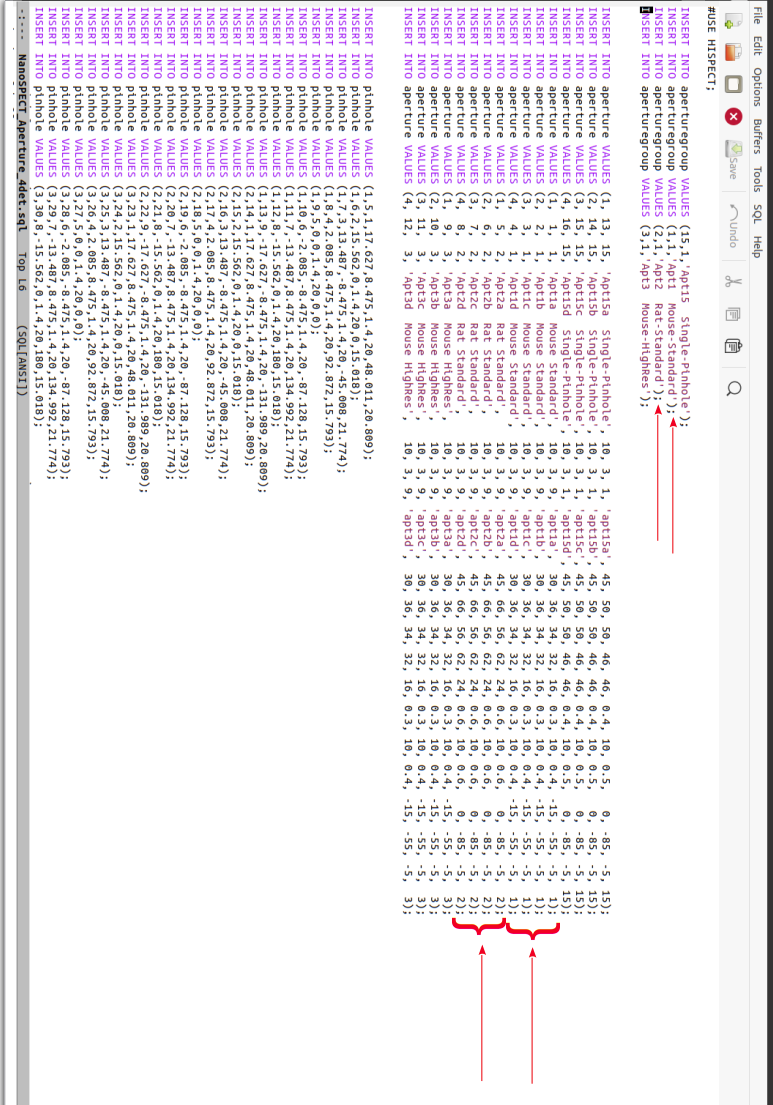
\includegraphics[scale=0.45]{figs/HiSPECT4det.png}
\caption{Part of \texttt{NanoSPECT\_Aperture\_4det.sql} file with important lines highlighted}
\label{fig:HiSPECT4det}
\end{figure}

\begin{figure}[htp]
\centering
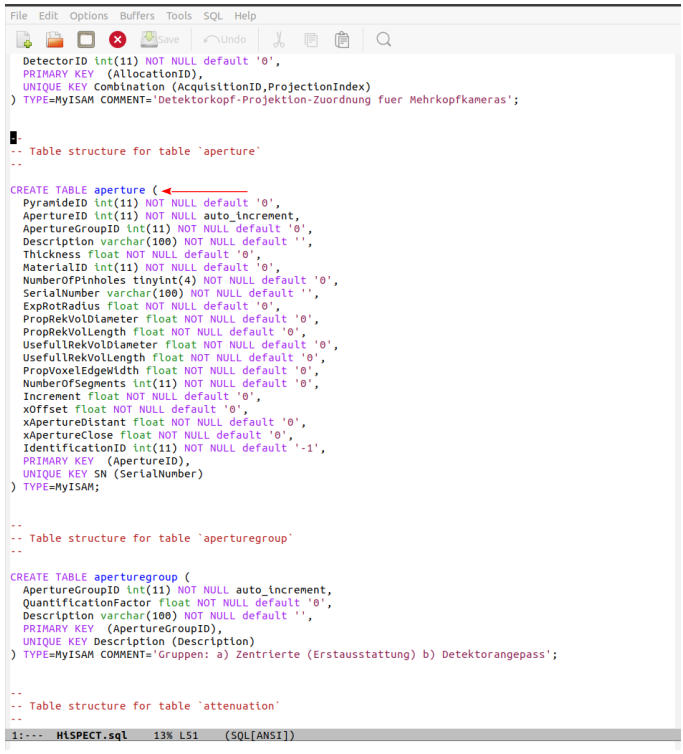
\includegraphics[scale=0.6]{figs/HiSPECTaperture.png}
\caption{Part of \texttt{HiSPECT.sql} file with important lines highlighted}
\label{fig:HiSPECTaperture}
\end{figure}


\begin{figure}[htp]
\centering
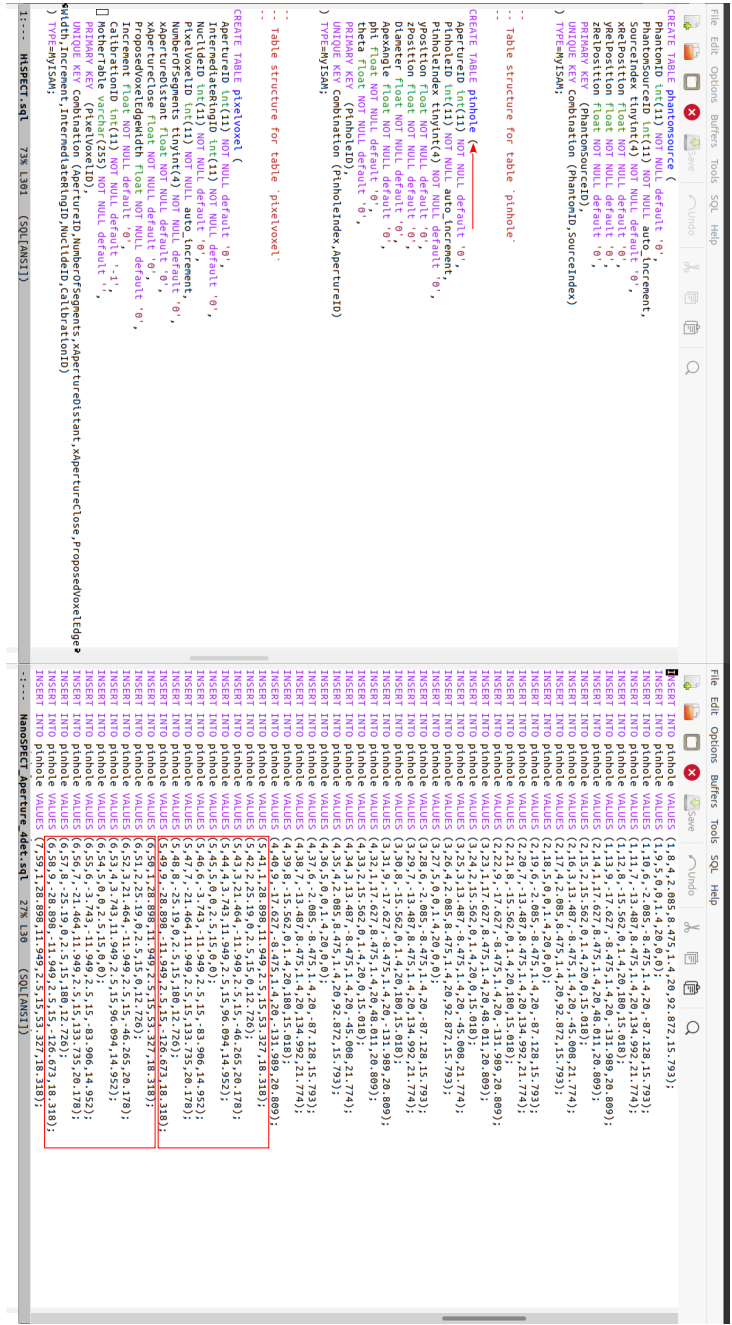
\includegraphics[scale=0.45]{figs/HiSPECTpinhole.png}
\caption{Part of \texttt{HiSPECT.sql} and \texttt{NanoSPECT\_Aperture\_4det.sql} file with important lines highlighted: parameters for APT1 are in blue rectangles and in red for APT2.}
\label{fig:HiSPECTpinhole}
\end{figure}

\clearpage
\subsection{HiSPECTtoGate tool}
This tool can be found on github: \href{https://github.com/kochebina/ParametrisedPinholeCollimator/tree/main/HiSPECTtoGATE}{HiSPECTtoGATE on github}. We decided to keep this script as simple as possible and not introduce the previous parameters as input options, thus, the script doesn't need a compilation. It is most probably will be used for inspiration.

It is important to notice that one should change some of lines of the script in order to adapt it for specific needs:
\begin{itemize}
\item line 16: give the name of your input file
\item line 22: give the rotation radius
\end{itemize}

In order to run the script one can simple does:   
\begin{verbatim}
root -l HiSPECTtoGate.C
\end{verbatim}

\subsection{Input file}
As input one should provide information from a text file obtained from HiSPECT (Figure~\ref{fig:HiSPECTpinhole}) ApertureName.hispect, for example APT1.hispect and APT2.hispect. These are text files produced "by hand". APT1.hispect and APT2.hispect are presented in Figure~\ref{fig:hispect}. 

The output files, APT1\_hispect.pin and APT2\_hispect.pin (Figure~\ref{fig:pin}), can be used directly in GATE macros.

\begin{figure}[htp]
\centering
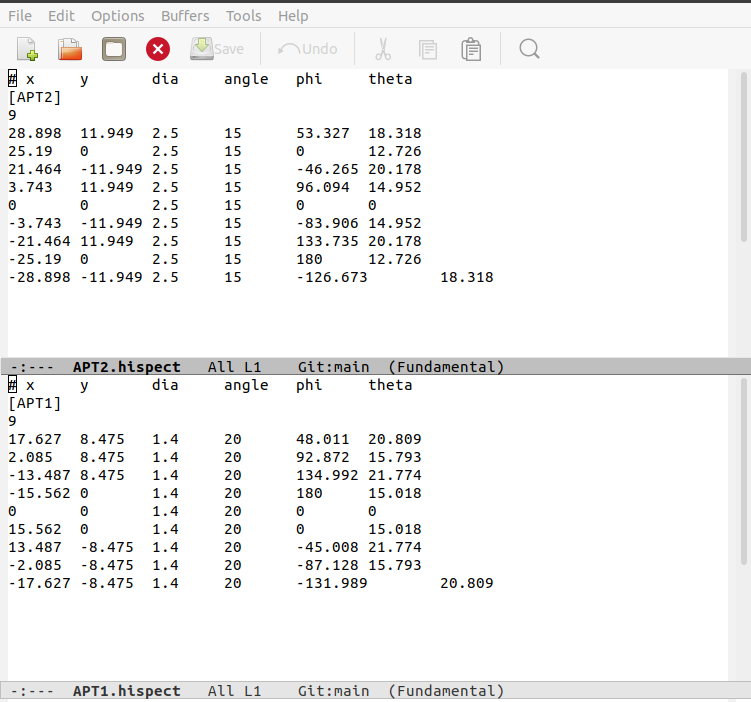
\includegraphics[scale=0.45]{figs/hispect.png}
\caption{APT1.hispect and APT2.hispect}
\label{fig:hispect}
\end{figure}

\begin{figure}[htp]
\centering
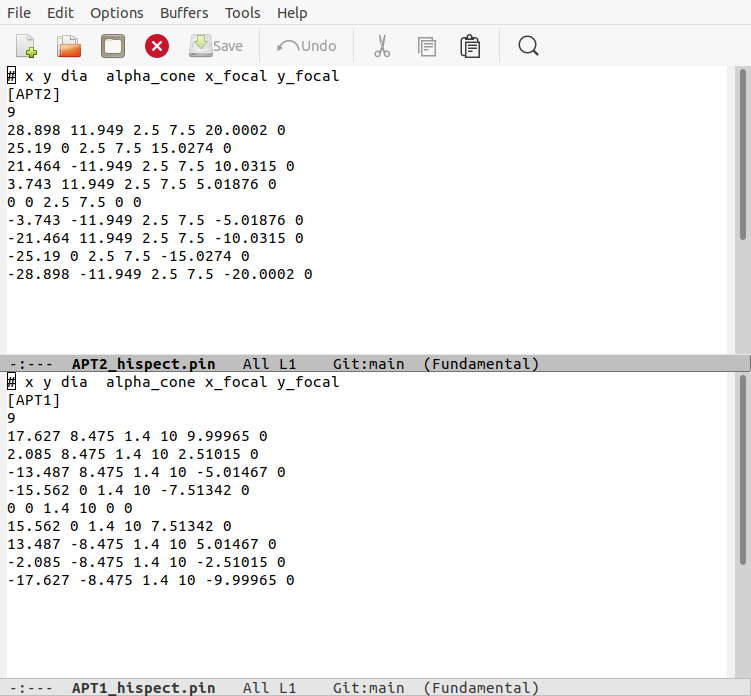
\includegraphics[scale=0.45]{figs/pin.png}
\caption{APT1\_hispect.pin and APT2\_hispect.pin produced by HiSPECTtoGate script and used in macros examples \href{https://github.com/kochebina/ParametrisedPinholeCollimator/tree/main/macros}{here}.}
\label{fig:pin}
\end{figure}
 





%\bibliographystyle{plain}
%\bibliography{biblio}



\end{document}
